\documentclass[11pt]{article}

\usepackage[margin=0.82in]{geometry}
\usepackage[T1]{fontenc}
\usepackage[utf8]{inputenc}
\usepackage{lmodern}
\usepackage{amsmath,amssymb}
\usepackage{array}
\usepackage{booktabs}
\usepackage{enumitem}
\usepackage{graphicx}
\usepackage{xcolor}
\usepackage{hyperref}
\usepackage{tikz}
\usepackage{tcolorbox}
\usepackage{longtable}
\usetikzlibrary{arrows.meta,positioning,shapes.geometric}

\hypersetup{
  colorlinks=true,
  linkcolor=blue!55!black,
  urlcolor=blue!55!black,
  citecolor=blue!55!black
}

\setlist[itemize]{topsep=2pt,itemsep=2pt,leftmargin=*}
\setlist[enumerate]{topsep=2pt,itemsep=2pt,leftmargin=*}
\renewcommand{\arraystretch}{1.18}

\definecolor{BOBlue}{RGB}{0,64,128}
\definecolor{SoftBlue}{RGB}{235,244,255}
\definecolor{SoftGray}{RGB}{246,246,246}
\definecolor{SoftGreen}{RGB}{238,248,239}
\definecolor{SoftRed}{RGB}{255,241,241}

\newtcolorbox{keybox}[1]{
  colback=SoftBlue,
  colframe=BOBlue,
  title=\textbf{#1},
  arc=2mm,
  boxrule=0.6pt
}

\newtcolorbox{answerbox}[1]{
  colback=SoftGreen,
  colframe=green!40!black,
  title=\textbf{#1},
  arc=2mm,
  boxrule=0.6pt
}

\newtcolorbox{warningbox}[1]{
  colback=SoftRed,
  colframe=red!55!black,
  title=\textbf{#1},
  arc=2mm,
  boxrule=0.6pt
}

\newcommand{\principle}[1]{\textbf{\textcolor{BOBlue}{#1}}}
\newcommand{\q}[1]{\paragraph{Question.} #1}
\newcommand{\ans}[1]{\paragraph{Strong answer.} #1}

\title{\textbf{Blue Origin Panel Interview Preparation Guide}\\
\large Data Acquisition and Controls Engineer II -- New Glenn, R66427}
\author{Interview Study Notes}
\date{\today}

\begin{document}
\maketitle

\begin{abstract}
This guide organizes technical and behavioral preparation for a Data Acquisition
and Controls Engineer II panel interview supporting New Glenn component testing.
The central theme is the ability to translate test objectives into safe,
traceable, maintainable measurement-and-control systems: sensor selection,
signal conditioning, acquisition, automated controls, interlocks, data
validation, post-processing, and engineering review.
\end{abstract}

\begin{keybox}{Core interview message}
``I can translate test objectives into a safe, traceable, and maintainable
measurement-and-control system--from sensor selection and signal conditioning
through acquisition, automated control, data validation, post-processing, and
engineering review.''
\end{keybox}

\tableofcontents
\newpage

\section{Role Understanding}

\subsection{Core engineering mission}
The role sits at the intersection of instrumentation, data acquisition, controls,
electrical integration, test software, and engineering analysis. The panel is
likely evaluating whether the candidate can build reliable test capability, not
merely write code.

\begin{center}
\resizebox{0.96\linewidth}{!}{%
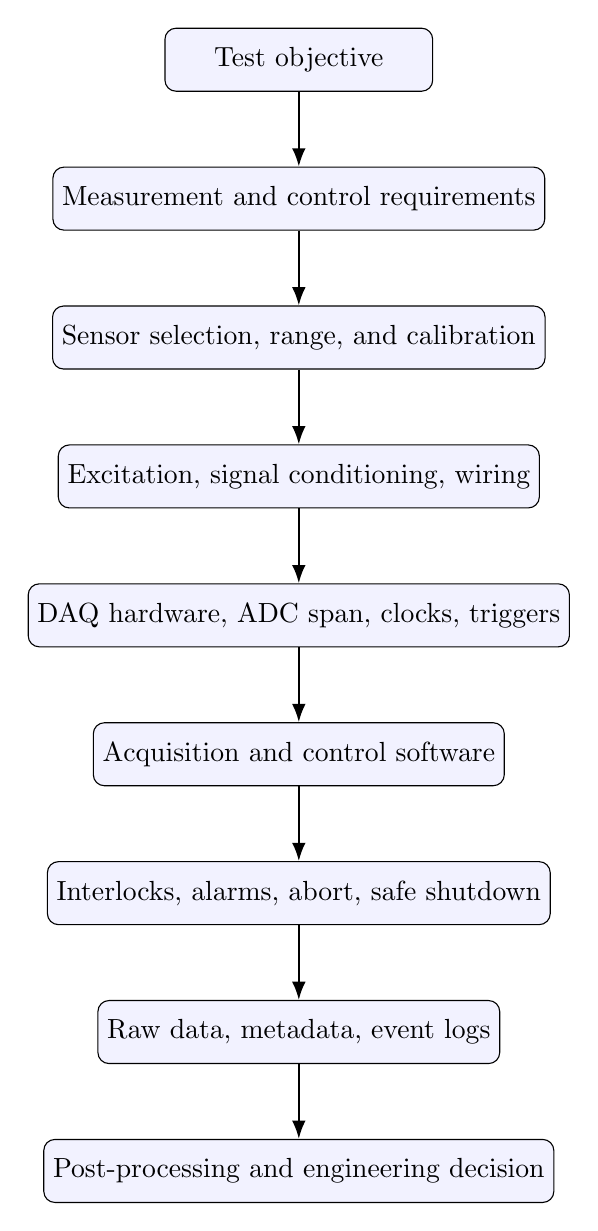
\begin{tikzpicture}[node distance=0.95cm,>=Latex]
  \tikzstyle{block}=[draw,rounded corners,align=center,minimum width=3.4cm,minimum height=0.8cm,fill=blue!5]
  \node[block] (obj) {Test objective};
  \node[block,below=of obj] (req) {Measurement and control requirements};
  \node[block,below=of req] (sensor) {Sensor selection, range, and calibration};
  \node[block,below=of sensor] (signal) {Excitation, signal conditioning, wiring};
  \node[block,below=of signal] (daq) {DAQ hardware, ADC span, clocks, triggers};
  \node[block,below=of daq] (sw) {Acquisition and control software};
  \node[block,below=of sw] (safe) {Interlocks, alarms, abort, safe shutdown};
  \node[block,below=of safe] (data) {Raw data, metadata, event logs};
  \node[block,below=of data] (review) {Post-processing and engineering decision};
  \foreach \a/\b in {obj/req,req/sensor,sensor/signal,signal/daq,daq/sw,sw/safe,safe/data,data/review}
    \draw[->,thick] (\a) -- (\b);
\end{tikzpicture}}
\end{center}

\subsection{What the panel is hiring you to do}
\begin{itemize}
  \item Convert test requirements into instrumentation and control plans.
  \item Select, integrate, calibrate, and validate sensors.
  \item Design or review signal-conditioning, grounding, shielding, wiring, and electrical interfaces.
  \item Configure DAQ hardware, clocks, triggers, ADC ranges, and acquisition software.
  \item Develop automated and semi-automated control logic.
  \item Ensure fail-safe operation, interlocks, alarms, and safe shutdown behavior.
  \item Store reliable, traceable, time-aligned data with useful metadata.
  \item Reduce, visualize, and review large datasets.
  \item Troubleshoot hardware/software problems under schedule pressure.
  \item Document systems so another engineer can operate and maintain them.
\end{itemize}

\subsection{Engineer II expectations}
At this level, expect questions that test independent execution, judgment, and
cross-disciplinary troubleshooting. The panel will likely expect you to:
\begin{itemize}
  \item Execute scoped work independently and identify unclear requirements.
  \item Make defensible technical decisions and explain tradeoffs.
  \item Troubleshoot across sensors, wiring, DAQ, software, controls, and data analysis.
  \item Escalate appropriately when safety, authority, or requirements are unclear.
  \item Communicate with test, mechanical, electrical, fluids, controls, and analysis engineers.
  \item Produce maintainable solutions rather than one-off scripts.
  \item Demonstrate safety judgment without exaggerating expertise.
\end{itemize}

\section{Likely Panel Structure}

The interview loop may include a hiring manager, DAQ/test software engineer,
controls engineer, instrumentation or electrical engineer, test operations
engineer, cross-functional stakeholder, and behavioral interviewer.

\begin{longtable}{p{0.29\linewidth}p{0.64\linewidth}}
\toprule
\textbf{Category} & \textbf{What to prepare} \\
\midrule
Resume/project deep dive & Your individual contribution, architecture decisions, failures, validation, and measurable impact. \\
DAQ and instrumentation & Sensors, signal conditioning, sampling, aliasing, ADCs, clocks, triggers, uncertainty. \\
Controls/test automation & State machines, PID, interlocks, watchdogs, aborts, commissioning, deterministic timing. \\
Python/software & Modular design, hardware abstraction, logging, testing, concurrency, data persistence. \\
Electrical troubleshooting & Schematics, grounding, shielding, noise, return paths, isolation, terminal wiring. \\
Data analysis & Traceability, filtering, time alignment, pass/fail metrics, metadata, reports. \\
Leadership Principles & STAR stories tied to ownership, safety, operational excellence, trust, and backbone. \\
Mission motivation & Why Blue Origin, why New Glenn, why this specific end-to-end test role. \\
\bottomrule
\end{longtable}

\section{Sixty-to-Ninety Second Introduction}

\subsection{Recommended structure}
\begin{enumerate}
  \item Current technical identity.
  \item Two or three capabilities relevant to DAQ, controls, test software, and analysis.
  \item One representative accomplishment with measurable impact.
  \item Why this position is the logical next step.
  \item Why Blue Origin and New Glenn.
\end{enumerate}

\begin{answerbox}{Model introduction}
``I am an engineer focused on real-time simulation, controls, test automation,
and data-driven system validation. In my current work, I support real-time
simulation environments where software, instrumentation, timing, and system
behavior must remain synchronized and reliable.

A representative example is a project where I developed or improved an
automated test and analysis workflow for [system]. I integrated
[hardware/software], implemented validation and fault detection, and improved
[test time, reliability, repeatability, or data quality] by [measured result].

This Blue Origin position is attractive because it combines the areas I most
enjoy: instrumentation, Python development, real-time systems, controls, test
execution, and troubleshooting. I am motivated by the direct connection between
test-data integrity and safe, repeatable flight hardware, and I would like to
bring my real-time simulation and automation experience into component testing
for New Glenn.''
\end{answerbox}

\section{DAQ Fundamentals}

\subsection{Sensor selection}
When selecting a sensor, discuss:
\begin{itemize}
  \item Range, proof pressure, burst pressure, over-range behavior, and fault margin.
  \item Accuracy, precision, repeatability, linearity, hysteresis, drift, and total uncertainty.
  \item Sensitivity, resolution, signal-to-noise ratio, and usable span.
  \item Bandwidth, dynamic response, mounting effects, and sensor loading.
  \item Environmental rating, fluid compatibility, calibration, and failure modes.
\end{itemize}

\begin{warningbox}{Range tradeoff}
A very large range may survive the test but provide poor useful resolution.
A tight range may improve resolution but fail to capture transients or fault
conditions. Selection should be tied to measurement objective and credible
off-nominal behavior.
\end{warningbox}

\subsection{Important sensor types}
\begin{longtable}{p{0.21\linewidth}p{0.71\linewidth}}
\toprule
\textbf{Sensor} & \textbf{Topics to know} \\
\midrule
Pressure transducer & Absolute, gauge, sealed gauge, differential; voltage and current outputs; proof/burst pressure; fluid compatibility; temperature effects; static versus dynamic measurement; tubing effects. \\
Thermocouple & Seebeck effect; type selection; cold-junction compensation; low-level voltage; extension wire compatibility; grounded versus ungrounded junctions; noise; response time; open detection. \\
RTD & Two-, three-, four-wire measurements; lead resistance; excitation current; self-heating; accuracy and stability; differences from thermocouples. \\
Load cell/strain gauge & Wheatstone bridges; quarter/half/full bridge; excitation; mV/V sensitivity; shunt calibration; temperature compensation; preload; load path; cable shielding; zero balance; creep. \\
\bottomrule
\end{longtable}

\subsection{Sensor-selection question}
\q{You need to measure pressure expected near 2,000 psi, but short transients
could reach 2,600 psi. How would you select the transducer?}

\ans{First clarify required accuracy, frequency content, fluid compatibility,
temperature, proof pressure, burst pressure, and whether the desired pressure is
absolute, gauge, sealed gauge, or differential. Do not select a 2,000 psi device
just because that is the nominal operating point. Choose a range that safely
captures credible transients while preserving useful resolution, possibly around
3,000 psi depending on uncertainty and safety margins. Then evaluate total
measurement uncertainty: sensor accuracy, temperature effects, signal
conditioning, ADC accuracy, calibration, mounting, and dynamic pressure-line
effects. Define over-range behavior, calibration requirements, and reasonableness
checks against related measurements.}

\q{What if the pressure has a high-frequency oscillation?}
\ans{Evaluate transducer frequency response and the dynamics introduced by tubing,
cavities, and mounting. Tubing can damp or resonate, so a high DAQ sample rate
alone does not ensure faithful measurement. Clarify whether the objective is mean
pressure, transient pressure, or oscillation characterization because each can
drive different sensor, mounting, and sampling choices.}

\section{Signal Conditioning, ADCs, and Sampling}

\subsection{Signal conditioning}
Prepare to explain amplification, attenuation, anti-alias filtering, isolation,
sensor excitation, bridge completion, cold-junction compensation, linearization,
current-to-voltage conversion, terminal configuration, common-mode voltage,
common-mode rejection, input impedance, ground loops, shielding, and cable
routing.

\begin{keybox}{Examples}
\begin{itemize}
  \item A load cell with 2 mV/V sensitivity and 10 V excitation produces only
  20 mV at rated load, so it normally requires low-noise differential measurement
  and appropriate gain.
  \item A 4--20 mA pressure transmitter can be useful in long-cable or noisy
  environments because current loops are robust and can indicate some open-circuit
  or under-range conditions.
\end{itemize}
\end{keybox}

\subsection{Sampling and aliasing}
Nyquist says the sample rate must exceed twice the highest frequency component
of interest. Practical engineering requires more: anti-alias filters are not
ideal, transients may require more samples per event, and synchronized channels
may impose timing constraints. Consider:
\begin{itemize}
  \item Highest physical signal frequency of interest and unwanted high-frequency content.
  \item Analog anti-alias filter cutoff, order, roll-off, and phase behavior.
  \item Desired time-domain fidelity and channel synchronization.
  \item Data volume, storage, network bandwidth, and control-loop timing.
  \item Hardware-timed versus software-timed acquisition.
\end{itemize}

\q{A sensor contains meaningful content up to 100 Hz. What sampling rate would you use?}
\ans{The theoretical lower limit is greater than 200 samples/s, but the rate should
not be selected from Nyquist alone. Review anti-alias filter cutoff and roll-off,
transient fidelity, time-alignment needs, control requirements, and storage
constraints. A rate such as 1 kS/s may be reasonable for good time-domain
representation, provided unwanted content above Nyquist is attenuated before
digitization.}

\begin{warningbox}{Weak answer to avoid}
``Exactly 200 Hz because Nyquist says twice the frequency.'' This ignores
realizable filters, guard band, timing fidelity, and unwanted high-frequency
content.
\end{warningbox}

\subsection{ADC fundamentals}
\q{What determines the smallest voltage change an ADC can represent?}
\ans{The ideal quantization step is the selected input span divided by the number
of ADC codes. For an \(N\)-bit ADC, there are nominally \(2^N\) codes. Effective
resolution is also affected by noise, gain error, offset, nonlinearity, reference
stability, front-end configuration, and sensor usable span. Distinguish ideal bit
resolution from effective number of bits and overall measurement uncertainty.}

\q{What is the difference between accuracy and resolution?}
\ans{Resolution is the smallest representable increment. Accuracy is closeness to
the true value. A system can display many digits while still being inaccurate due
to offset, drift, calibration error, sensor error, electrical noise, or poor
installation.}

\section{Grounding, Shielding, and Noise Troubleshooting}

\subsection{Topics to review}
Ground loops, common-mode noise, differential inputs, single-point grounding,
shield termination, twisted pairs, sensor/power separation, electromagnetic
interference, isolation, cable length/capacitance, chassis ground versus signal
common, 50/60 Hz pickup, switching noise, and thermocouple grounding problems.

\begin{warningbox}{Do not over-generalize}
``Ground the shield at one end'' is not a universal law. The correct shield
strategy depends on frequency, system architecture, isolation, chassis bonding,
safety grounding, and manufacturer guidance.
\end{warningbox}

\q{A pressure measurement is stable when the pump is off but noisy when the pump starts. How would you troubleshoot it?}
\ans{First keep the system safe and avoid changing multiple variables at once.
Characterize the noise: amplitude, frequency, affected channels, and correlation
with pump speed, switching, or flow conditions. Separate possible causes into
real pressure pulsation, electrical interference, grounding, mechanical
vibration, signal-conditioning saturation, and software configuration. Compare
nearby sensors, inspect raw data rather than only filtered trends, check shield
and ground continuity, review cable routing near motor power, and measure the
signal at successive points in the chain. Substitute a known signal or simulator
at the DAQ input. If clean, focus upstream; if noisy, focus on conditioning,
cabling, grounding, or DAQ setup. Document each change. Do not use a digital
filter to hide an unresolved physical or electrical issue. Also verify that
``noise'' is not legitimate pressure pulsation important to hardware safety.}

\section{Controls and Automated Test Operations}

\subsection{Control-system fundamentals}
Review open-loop versus closed-loop control, PID, stability, overshoot, settling
time, sensor delay, actuator saturation, integrator windup, rate limiting,
setpoint ramping, discrete-time implementation, control-loop frequency, state
machines, fault states, interlocks, permissives, watchdogs, emergency shutdown,
manual/automatic modes, bumpless transfer, and determinism.

\subsection{State-machine design}
\begin{center}
\resizebox{0.96\linewidth}{!}{%
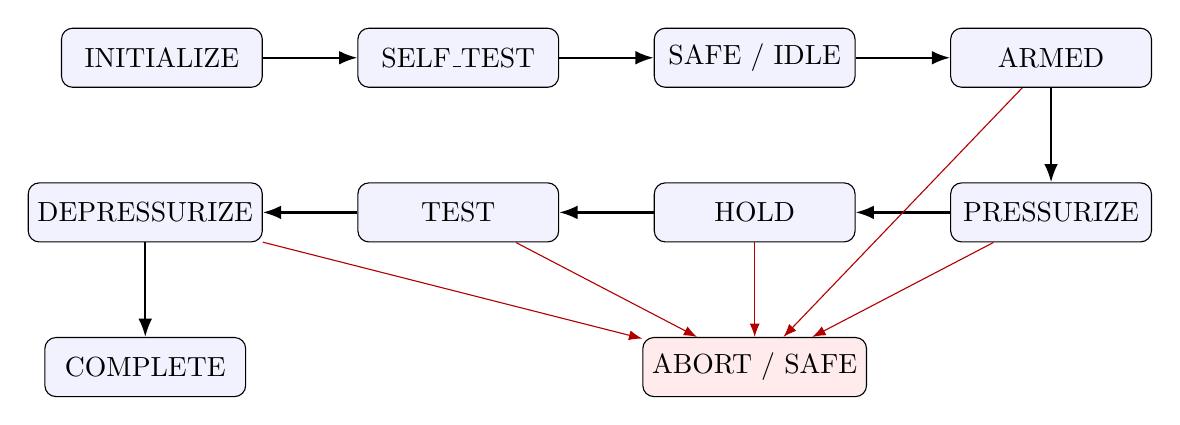
\begin{tikzpicture}[node distance=1.2cm,>=Latex]
  \tikzstyle{state}=[draw,rounded corners,align=center,minimum width=2.55cm,minimum height=0.75cm,fill=blue!5]
  \node[state] (init) {INITIALIZE};
  \node[state,right=of init] (self) {SELF\_TEST};
  \node[state,right=of self] (safe) {SAFE / IDLE};
  \node[state,right=of safe] (armed) {ARMED};
  \node[state,below=of armed] (press) {PRESSURIZE};
  \node[state,left=of press] (hold) {HOLD};
  \node[state,left=of hold] (test) {TEST};
  \node[state,left=of test] (dep) {DEPRESSURIZE};
  \node[state,below=of hold,fill=red!8] (abort) {ABORT / SAFE};
  \node[state,below=of dep] (complete) {COMPLETE};
  \draw[->,thick] (init) -- (self);
  \draw[->,thick] (self) -- (safe);
  \draw[->,thick] (safe) -- (armed);
  \draw[->,thick] (armed) -- (press);
  \draw[->,thick] (press) -- (hold);
  \draw[->,thick] (hold) -- (test);
  \draw[->,thick] (test) -- (dep);
  \draw[->,thick] (dep) -- (complete);
  \foreach \s in {armed,press,hold,test,dep}
    \draw[->,thin,red!70!black] (\s) -- (abort);
\end{tikzpicture}}
\end{center}

For every state define entry conditions, permissives, commands, expected sensor
responses, timeouts, exit conditions, fault triggers, safe-state actions,
operator authority, and logged events.

\q{Design the control architecture for an automated pressure test.}
\ans{Begin by clarifying hardware, pressure range, test medium, credible hazards,
ramp profile, hold duration, leakage limits, abort criteria, and safety
criticality. Implement an explicit state machine rather than an unstructured
sequence. Before arming, verify sensor health, communications, valve positions,
pressure boundaries, emergency-stop status, and environmental conditions. During
pressurization, apply a controlled ramp with high-pressure, high-rate-of-rise,
sensor-disagreement, timeout, valve-response, and communication-loss checks.
Safety-critical shutdown should not depend solely on a non-deterministic user
interface. Where required by hazard analysis, protection belongs in independent
hardware or a dedicated safety layer. Timestamp every command, state transition,
interlock, and operator action. Define safe behavior for power loss, communication
loss, invalid data, and software failure. Validate with simulation, dry runs,
fault injection, and low-energy commissioning before full conditions.}

\q{A pressure-control loop oscillates around the setpoint. What could cause it?}
\ans{Possible causes include excessive proportional or integral gain, insufficient
damping, sensor noise, process delay, actuator deadband, valve stiction,
saturation, incorrect loop timing, unit errors, or operation away from the tuning
point. Review trends for setpoint, measurement, error, controller output, valve
feedback, and saturation. Verify timing and units before retuning. If the
actuator is saturating, review anti-windup and command limits.}

\section{Test Safety and Fault Management}

\subsection{Safety hierarchy}
Use layered protection:
\begin{enumerate}
  \item Inherently safer design.
  \item Physical limits and protective hardware.
  \item Independent interlocks.
  \item Control software protections.
  \item Procedural controls.
  \item Operator training and personal protective equipment.
\end{enumerate}

\begin{warningbox}{Important safety statement}
A Python exception handler is not a substitute for independent overpressure
protection, emergency-stop chains, relief devices, or a safety-rated control
layer when the hazard analysis requires them.
\end{warningbox}

\q{What should the test stand do if communication with the controller is lost?}
\ans{The correct behavior must come from the hazard analysis and safe-state
definition. Do not assume holding the last command is safe. Outputs should
transition predictably under communication loss, watchdog timeout, application
failure, and power loss. Critical protection should remain effective even if the
supervisory application is unavailable.}

\q{You are close to a scheduled test, but an interlock is producing intermittent trips. What do you do?}
\ans{Do not bypass a safety interlock simply to preserve schedule. Pause,
characterize the fault, and determine whether the trip is a real unsafe
condition, instrumentation fault, configuration error, or interlock implementation
issue. Engage responsible disciplines. A temporary configuration, if allowed at
all, requires documented risk evaluation and authorization. Schedule pressure
does not change physical risk.}

\section{Python and Software Engineering}

\subsection{Topics to prepare}
Classes, modules, type hints, exceptions, context managers, logging, unit tests,
mocking hardware interfaces, configuration management, concurrency, threads
versus processes, queues, async I/O, NumPy, pandas, plotting, file formats, data
validation, profiling, packaging, Git, code review, and continuous integration.

\subsection{Recommended DAQ software architecture}
\begin{center}
\resizebox{0.92\linewidth}{!}{%
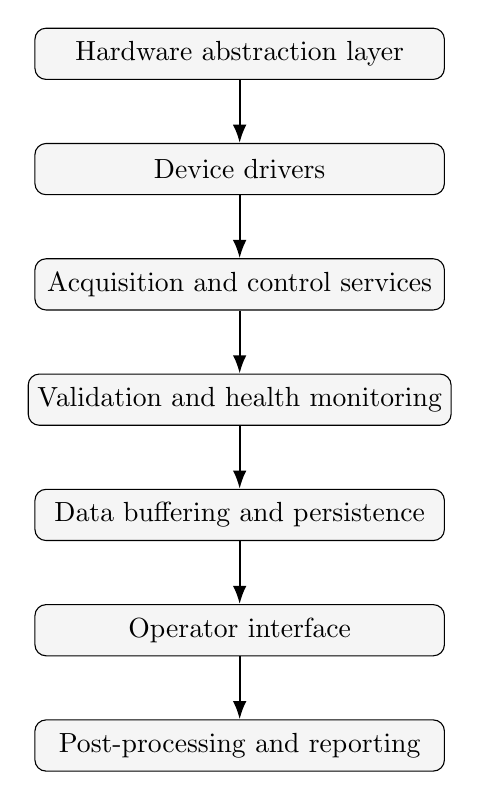
\begin{tikzpicture}[node distance=0.8cm,>=Latex]
  \tikzstyle{layer}=[draw,rounded corners,align=center,minimum width=5.2cm,minimum height=0.65cm,fill=gray!8]
  \node[layer] (hal) {Hardware abstraction layer};
  \node[layer,below=of hal] (drivers) {Device drivers};
  \node[layer,below=of drivers] (services) {Acquisition and control services};
  \node[layer,below=of services] (health) {Validation and health monitoring};
  \node[layer,below=of health] (persist) {Data buffering and persistence};
  \node[layer,below=of persist] (ui) {Operator interface};
  \node[layer,below=of ui] (post) {Post-processing and reporting};
  \foreach \a/\b in {hal/drivers,drivers/services,services/health,health/persist,persist/ui,ui/post}
    \draw[->,thick] (\a) -- (\b);
\end{tikzpicture}}
\end{center}

Benefits: hardware can be mocked, UI failures need not stop acquisition, scaling
and calibration are centralized, drivers can be replaced, and fault handling is
easier to verify.

\q{How would you design Python software to acquire 100 channels continuously?}
\ans{Start with sample rates, synchronization, latency, data volume, acceptable
loss, and hardware-driver constraints. Separate acquisition from visualization
and disk writing so slow UI or file operations cannot block time-critical reads.
Acquisition should place timestamped blocks into bounded queues or ring buffers.
A persistence worker writes chunked data and metadata; a display path decimates
independently. Monitor queue depth, dropped samples, hardware status, timing
errors, and disk capacity. Use versioned configuration files, structured logs,
graceful shutdown, and automatic file finalization. Test with simulated devices,
long-duration soak tests, injected failures, and known waveforms before
commissioning with hardware.}

\q{What happens if the disk writer falls behind?}
\ans{Define behavior deliberately. Monitor buffer occupancy and warn early.
Depending on test criticality, the system might abort safely before data loss,
reduce nonessential display processing, or temporarily absorb backlog in a
bounded buffer. Do not permit silent data loss.}

\section{NI Hardware, LabVIEW, and DAQmx}

\subsection{Concepts to review}
NI CompactDAQ versus PXI/PXIe, multifunction DAQ devices, analog input/output,
digital I/O, counter/timer channels, hardware-timed and software-timed
acquisition, sample clocks, start triggers, reference triggers, module
synchronization, buffered tasks, regeneration, DAQmx tasks/channels, terminal
configuration, continuous versus finite sampling, LabVIEW producer-consumer
architecture, LabVIEW state machines, Real-Time, and FPGA concepts.

\q{What is the advantage of hardware-timed acquisition?}
\ans{Hardware timing uses DAQ timing resources rather than relying on
operating-system scheduling for every sample. It provides more consistent sample
intervals and better synchronization. The host application transfers blocks of
samples while the hardware sample clock determines acquisition timing.}

\q{How should you answer if your LabVIEW experience is limited?}
\ans{Be direct: ``My direct experience is stronger in Python and real-time
simulation than in LabVIEW. However, I understand the core DAQ concepts--tasks,
channels, clocks, triggers, buffering, scaling, and synchronized acquisition. I
have also worked with modular software and state-machine architectures, so I
would transfer those principles while learning Blue's established design
patterns and code-review expectations.''}

\section{Data Processing, Validation, and Visualization}

\subsection{Robust post-processing pipeline}
A robust pipeline should:
\begin{itemize}
  \item Read raw data without altering it and verify file integrity.
  \item Load calibration and configuration versions.
  \item Convert to engineering units and preserve raw samples.
  \item Handle invalid or missing samples explicitly.
  \item Align channels in time and detect the relevant test interval.
  \item Apply justified filtering with documented parameters.
  \item Calculate metrics, propagate quality flags, and generate plots/reports.
  \item Preserve traceability to raw data, procedure, configuration, and software revision.
\end{itemize}

\q{How would you determine whether a component passed a test?}
\ans{Do not rely on a single opaque pass/fail calculation. Define acceptance
criteria with the responsible engineering authority. Identify exact channels and
time intervals, verify data quality, and compute each metric with units and
uncertainty. The output should show result, limit, margin, quality status, and
traceability to raw data, configuration, calibration, and analysis-code version.
If required channels are invalid, the correct result may be ``indeterminate''
rather than pass or fail.}

\q{When is filtering appropriate?}
\ans{Filtering is appropriate when it follows from the physical measurement
objective and has documented characteristics. Preserve raw data; specify filter
type, order, cutoff, phase behavior, and edge handling. Do not choose a filter
only because the plot looks cleaner.}

\q{Two channels appear offset by 20 ms. What might cause it?}
\ans{Possible causes include separate sample clocks, unsynchronized devices,
software timestamps, channel multiplexing, filter group delay, transport
buffering, different sensor response times, or timestamp interpretation errors.
Establish whether the offset originates in physical sensors, acquisition
hardware, communication, or post-processing before shifting data.}

\section{Databases and Data Architecture}

\subsection{Concepts to know}
Raw waveform storage versus metadata storage, relational databases, time-series
databases, HDF5, TDMS, Parquet, binary files, indexing, schema design, data
retention, checksums, access control, configuration versioning, calibration
traceability, test identifiers, searchability, backup, and recovery.

\q{How would you organize test data?}
\ans{Separate immutable raw measurements from searchable test metadata. Each test
should have a unique identifier linked to the unit under test, procedure version,
software commit, DAQ configuration, channel map, calibration records, operator,
timestamps, and environmental conditions. Large waveform data may belong in a
structured file or object store, while a relational database indexes the test and
metadata. The architecture should let an engineer reproduce how an
engineering-unit value and final metric were generated.}

\section{Electrical Schematics and Wiring Diagrams}

\subsection{What to review}
Power distribution, voltage rails, fuses, breakers, relays, contactors,
grounding, terminal blocks, connector pinouts, cable and wire identifiers,
analog and digital signal paths, normally open/closed contacts, interlocks,
emergency-stop chains, shield termination, sensor excitation, return paths, and
isolation boundaries.

\q{A sensor reads full scale regardless of applied input. How would you diagnose it?}
\ans{Confirm the condition is safe and determine whether this is raw ADC saturation
or a software-scaled full-scale result. Inspect channel type, terminal mode,
input range, scaling, and excitation. Use the schematic to trace the signal from
sensor to terminal block, conditioner, connector, and DAQ input. Measure known
points with appropriate equipment. Inspect for open return, short to excitation,
wrong pinout, loss of bridge completion, common-mode violations, and scaling
errors. Apply a known simulator at the DAQ input to isolate sensor/wiring from
the acquisition chain.}

\section{Test Stand Commissioning}

\subsection{Progressive commissioning sequence}
\begin{enumerate}
  \item Design, hazard, schematic, and configuration review.
  \item Wiring inspection, continuity, isolation, and power-off verification.
  \item Controlled power-up and power rail verification.
  \item I/O checkout with known stimuli and sensor simulators.
  \item Actuator command/feedback tests under controlled conditions.
  \item Interlock, abort, permissive, and fault-injection verification.
  \item Dry run, low-energy test, and incremental envelope expansion.
  \item Readiness review, configuration baseline, and full test.
\end{enumerate}

\q{How would you commission a new test stand?}
\ans{Use a written commissioning plan with expected results and signoffs. Start
with drawing and configuration review, then verify wiring, grounding, power, and
protective devices before energization. Check every I/O channel with known
stimuli and verify engineering-unit scaling end to end. For outputs, test
commands under controlled conditions and confirm both command and independent
feedback. Exercise permissives, aborts, communication failures, sensor failures,
and power-loss behavior. Conduct dry runs and gradually increase test energy.
Track discrepancies to closure. The released baseline should include hardware,
software, channel map, calibration, and procedure versions.}

\section{Open-Ended System Design Exercise}

\subsection{Prompt}
``Design a DAQ and control system for testing a pressurized component.''

\subsection{Step 1: Clarify requirements}
Ask about the component, test objective, medium, normal and maximum pressures,
temperatures, required dynamics, channel count, safety-critical measurements,
controlled actions, timing accuracy, pass/fail criteria, safe state, redundancy,
duration, and applicable standards.

\subsection{Step 2: Define instrumentation}
Possible measurements include inlet/outlet pressure, differential pressure,
temperature, flow rate, load or strain, valve position, supply voltage/current,
ambient conditions, and vibration if relevant.

\subsection{Step 3: Build measurement chains}
For each channel define:
\[
\text{quantity} \rightarrow \text{sensor} \rightarrow \text{excitation}
\rightarrow \text{conditioning} \rightarrow \text{wiring/shielding}
\rightarrow \text{DAQ input} \rightarrow \text{scaling}
\rightarrow \text{quality check} \rightarrow \text{storage}.
\]

\subsection{Step 4: Define control architecture}
Include state machine, permissives, interlocks, setpoint ramps, timeouts,
watchdogs, abort logic, manual-mode restrictions, hardware safety layer, and
operator interface.

\subsection{Step 5: Define data architecture}
Include hardware timestamps, shared clocks/triggers, channel map, calibration
version, configuration version, raw and processed data, event log, operator log,
software commit, and test article serial number.

\subsection{Step 6: Define verification}
Include unit tests, integration tests, sensor simulators, known electrical
inputs, fault injection, latency tests, long-duration tests, data-recovery tests,
safe-shutdown tests, and an end-to-end dry run.

\section{Leadership Principles and STAR Preparation}

\subsection{Blue Origin principles to map}
Prepare flexible STAR stories for:
\begin{itemize}
  \item \principle{Passion for Our Mission}
  \item \principle{Customer Focus}
  \item \principle{Deliver Results}
  \item \principle{Embrace Team Blue}
  \item \principle{Resourceful}
  \item \principle{Bias for Action}
  \item \principle{Ownership}
  \item \principle{Operational Excellence}
  \item \principle{Earn the Trust of Others}
  \item \principle{Hire and Develop the Best}
  \item \principle{Insist on the Highest Standards}
  \item \principle{Technical Ambition and Simplicity}
  \item \principle{Practice Humility}
  \item \principle{Have Backbone; Disagree and Commit}
\end{itemize}

\subsection{STAR structure}
\begin{longtable}{p{0.18\linewidth}p{0.18\linewidth}p{0.56\linewidth}}
\toprule
\textbf{Part} & \textbf{Share} & \textbf{Content} \\
\midrule
Situation & 10--15\% & Give only context needed to understand the problem. \\
Task & 10--15\% & State your responsibility and desired outcome. \\
Action & 55--65\% & Explain what you personally did, decisions, alternatives, risks, collaboration, and validation. \\
Result & 15--20\% & Include measurable result, safety/quality impact, lesson learned, and lasting mechanism. \\
\bottomrule
\end{longtable}

\section{Behavioral Questions and Model Answers}

\subsection{Ownership}
\q{Tell me about a problem outside your formal responsibility that you took ownership of.}
\ans{Situation: repeated failures were treated as isolated software issues while
ownership was split across teams. Task: your assigned area was narrower, but the
interface problem threatened schedule and reliability. Action: you created an
end-to-end signal map, gathered controls/hardware/test stakeholders, reproduced
the issue, isolated root cause, documented assumptions, implemented the fix, and
added an automated pre-test check. Result: failure rate dropped from [X] to [Y],
the team recovered [time], and the diagnostic became standard workflow.}

\subsection{Operational Excellence}
\q{Tell me about a recurring defect you eliminated.}
\ans{A recurring data-quality issue was being handled by reruns. You analyzed
history and found that a configuration, calibration, or timing condition was not
validated before acquisition. You added an automated preflight check,
configuration signature, and explicit failure message. The mechanism replaced
``be careful'' with prevention, reduced retests/manual effort by [amount], and
made remaining failures easier to diagnose.}

\subsection{Highest Standards and safety}
\q{Tell me about a time you stopped or delayed work because of a quality concern.}
\ans{Before a test/release, you found a mismatch between configured limits and an
approved requirement. Proceeding would meet schedule but create risk. You paused
the activity, collected evidence, involved responsible stakeholders, found root
cause, corrected the configuration, independently verified it, and resumed after
review. The delay prevented invalid or unsafe testing and led to a future
configuration-verification check.}

\subsection{Have Backbone; Disagree and Commit}
\q{Tell me about a time you disagreed with a technical decision.}
\ans{The team favored an approach that you believed introduced risk. You first
understood the opposing argument, then presented evidence comparing reliability,
timing, cost, safety, or maintainability. You proposed a small experiment to
resolve uncertainty. Whether your approach or the other approach won, you
committed to executing the final decision successfully.}

\subsection{Practice Humility}
\q{Tell me about a mistake.}
\ans{Use a real mistake, not a disguised strength. Explain the incorrect assumption,
impact, containment, communication, correction, and mechanism added to prevent
recurrence. End with a specific technical or communication lesson learned.}

\subsection{Deliver Results}
\q{Tell me about a project with an aggressive deadline.}
\ans{Reduce the work to critical deliverables, distinguish required functions from
enhancements, attack high-risk interfaces first, and use short validation
milestones. When setbacks occur, communicate early, adapt the approach, and
deliver the result without waiving required safety or validation steps.}

\subsection{Resourceful}
\q{Tell me about accomplishing something with limited tools or resources.}
\ans{If hardware or test access was unavailable, describe building a simulator,
replay tool, mock interface, or automated harness. State what it could and could
not validate. Explain how it enabled early testing, reduced integration time, and
became reusable.}

\subsection{Earn the Trust of Others}
\q{Tell me about working with a difficult stakeholder.}
\ans{Avoid labeling the person as difficult. Focus on conflicting objectives.
Understand concerns, summarize agreement, make interfaces explicit, follow
through on small commitments, share data openly, invite them into validation,
and complete the result even if every detail was not agreed upon.}

\section{Failure and Troubleshooting Questions}

\subsection{Common follow-ups}
Expect:
\begin{itemize}
  \item What exactly did you do versus what did the team do?
  \item Why did you choose that approach, and what alternatives did you reject?
  \item What data supported your conclusion?
  \item How did you validate the fix and prevent recurrence?
  \item What was the final root cause?
  \item What would you do differently?
  \item Did anyone disagree?
  \item What was the measurable result?
  \item What safety consequences existed?
  \item How did you know the result was correct?
\end{itemize}

\subsection{Troubleshooting framework}
\begin{enumerate}
  \item Make the condition safe.
  \item Define the symptom precisely and establish what changed.
  \item Reproduce the issue if safe and useful.
  \item Separate hardware, software, configuration, and physical causes.
  \item Change one variable at a time and instrument the diagnostic process.
  \item Test the hypothesis and validate the fix under representative conditions.
  \item Add a mechanism preventing recurrence.
  \item Document the outcome.
\end{enumerate}

\section{Mission and Motivation}

\q{Why Blue Origin?}
\ans{``I am interested in Blue Origin because the mission connects long-term space
access with engineering that must work safely and repeatedly. This role is
especially compelling because test-system quality directly affects whether
engineering teams can trust the evidence used to qualify hardware. My background
in [real-time simulation, controls, automation, Python, or instrumentation]
aligns with the full workflow described in the position--from acquiring
synchronized data and automating test operations to troubleshooting integration
issues and producing reliable engineering metrics. New Glenn presents the kind
of complex, multidisciplinary environment where I want to grow.''}

\q{Why New Glenn?}
\ans{``New Glenn interests me because reusability places a premium on consistent
testing, traceable data, and understanding hardware across repeated operating
cycles. A reusable vehicle requires not only successful operation but evidence
that components and systems remain within acceptable margins. I am motivated by
building test infrastructure that produces that evidence reliably.''}

\q{Why this specific position?}
\ans{``This position does not isolate software from hardware. It combines sensor
integration, electrical systems, DAQ architecture, controls, Python, data
processing, and test execution. That end-to-end responsibility is attractive
because I like understanding how a physical measurement becomes a trusted
engineering decision.''}

\section{Questions to Ask the Panel}

\subsection{Hiring manager}
\begin{itemize}
  \item What are the highest-priority test capabilities this engineer would support in the first six months?
  \item What differentiates an Engineer II who meets expectations from one who excels?
  \item Is the work primarily new test-system development, sustaining existing systems, or both?
  \item What are the team's largest technical bottlenecks today?
  \item How is ownership divided among test engineering, instrumentation, controls, software, and operations?
  \item What does commissioning and readiness review look like?
\end{itemize}

\subsection{DAQ/software engineer}
\begin{itemize}
  \item What DAQ platforms and software architectures are most common?
  \item How do you manage channel configuration, calibration, and metadata?
  \item How are software releases validated before use on hardware?
  \item How do you simulate hardware interfaces during development?
  \item What time-synchronization challenges are most important?
  \item How do you balance reusable frameworks with test-specific requirements?
\end{itemize}

\subsection{Controls/test-operations engineer}
\begin{itemize}
  \item How are safety-critical protections divided among hardware interlocks, real-time control, and supervisory software?
  \item What level of automation is typical during component testing?
  \item What are the most common causes of commissioning delays?
  \item How are off-nominal conditions and abort sequences validated?
  \item How much direct test execution and console support would this role perform?
\end{itemize}

\begin{answerbox}{Strong closing question}
``Based on our discussion, is there any part of my experience or technical
background that you would like me to clarify before we finish?''
\end{answerbox}

\section{One-Page Interview Summary Template}

\subsection*{Heading}
Data Acquisition and Controls Engineer II -- New Glenn

\subsection*{Understanding of the role}
This role develops and commissions component test systems for New Glenn,
integrating sensor instrumentation, DAQ hardware and software, automated
controls, data management, and post-processing. The central responsibility is to
produce reliable, traceable test evidence while supporting safe and repeatable
test operations.

\subsection*{Relevant capabilities}
\begin{itemize}
  \item Python development for automation and analysis.
  \item Real-time simulation or HIL systems.
  \item Controls and state-machine implementation.
  \item Instrumentation and synchronized acquisition.
  \item Electrical/software troubleshooting.
  \item Data processing, visualization, and validation.
  \item Git, testing, documentation, and configuration control.
\end{itemize}

\subsection*{Representative accomplishment}
Use one concise STAR example with a quantified result: problem, personal action,
validation, measured impact, and lasting mechanism.

\subsection*{Why Blue Origin and New Glenn}
Connect mission, reusable launch systems, safe human-capable architecture,
reliable test infrastructure, and your technical growth.

\subsection*{First-year contribution}
Aim to become productive in the team's DAQ and control architecture, own scoped
test-system improvements, strengthen automated validation/documentation, and
contribute dependable troubleshooting and commissioning support.

\section{Seven-Day Preparation Plan}

\begin{longtable}{p{0.12\linewidth}p{0.80\linewidth}}
\toprule
\textbf{Day} & \textbf{Focus} \\
\midrule
1 & Map job responsibilities and qualifications to real examples. Identify weakest two areas. Draft introduction, ``Why Blue Origin,'' and ``Why New Glenn.'' \\
2 & Review sensors, signal conditioning, ADC resolution, sampling, aliasing, filtering, uncertainty, calibration, noise, and grounding. Practice two system designs aloud. \\
3 & Review state machines, PID, interlocks, permissives, watchdogs, fail-safe design, aborts, commissioning, and fault insertion. Draw a pressure-test state machine from memory. \\
4 & Review Python architecture, hardware abstraction, threading/queues, logging, exceptions, unit/integration testing, persistence, Git, and configuration management. \\
5 & Review time-series processing, alignment, filtering, outliers, test metrics, traceability, DAQmx terms, hardware clocks/triggers, and LabVIEW architecture concepts. \\
6 & Write eight STAR stories. Map each to two or three principles. Practice two-minute and five-minute versions with numerical results and lessons. \\
7 & Run a 90-minute mock panel: intro, resume deep dive, DAQ, controls, troubleshooting, Python architecture, behavioral questions, your questions, and closing statement. \\
\bottomrule
\end{longtable}

\section{Final Interview Checklist}

\subsection{Technical}
\begin{itemize}
  \item Explain a complete sensor-to-database chain.
  \item Calculate ADC resolution conceptually.
  \item Explain practical sampling-rate selection and anti-alias filtering.
  \item Compare thermocouples and RTDs.
  \item Explain load-cell bridge measurements and shunt calibration.
  \item Troubleshoot grounding, shielding, and pump-correlated noise.
  \item Design a test state machine with interlocks, watchdogs, and safe state.
  \item Describe robust Python DAQ architecture.
  \item Explain hardware versus software timing.
  \item Describe commissioning, checkout, and fault injection.
  \item Explain traceability, calibration, uncertainty, and data quality flags.
\end{itemize}

\subsection{Behavioral}
\begin{itemize}
  \item Ownership story.
  \item Safety/high-standards story.
  \item Root-cause and operational-excellence story.
  \item Difficult technical problem.
  \item Failure and lesson learned.
  \item Conflict/disagreement.
  \item Tight deadline without compromising safety.
  \item Cross-functional collaboration.
  \item Resourcefulness.
  \item Mission motivation.
\end{itemize}

\subsection{Presentation}
\begin{itemize}
  \item 60--90 second introduction.
  \item Two-minute STAR versions with quantified outcomes.
  \item Clear distinction between ``I'' and ``we.''
  \item Five thoughtful questions.
  \item Concise closing statement.
\end{itemize}

\section{Recommended Closing Statement}

\begin{answerbox}{Closing statement}
``Thank you for the discussion. This role strongly matches the work I want to
continue developing--real-time systems, data acquisition, controls, test
automation, and engineering analysis. I am particularly interested in owning the
complete path from instrumented hardware to trusted test results. Based on what
I have learned, I believe my background in [your strongest two areas] would let
me contribute to the team while continuing to grow in [relevant area]. I am
excited about the opportunity to support safe and repeatable testing for New
Glenn.''
\end{answerbox}

\end{document}
